\documentclass[aspectratio=169,10pt]{beamer}

% -----------------------------------------------------------------------------
% Packages & Configuration
% -----------------------------------------------------------------------------
\usepackage[utf8]{inputenc}
\usepackage[T1]{fontenc}
\usepackage{lmodern}
\usepackage{amsmath,amssymb,amsfonts,bm}
\usepackage{booktabs,multirow}
\usepackage{graphicx}
\usepackage{xcolor}
\usepackage{tikz}
\usetikzlibrary{arrows.meta,positioning,shapes.geometric,fit,backgrounds,calc}
\usepackage{colortbl}
\usepackage{microtype}

% -----------------------------------------------------------------------------
% Color Palette: Academic FAU Navy + MIS Chair Teal + REHAU Brand Accent
% -----------------------------------------------------------------------------
\definecolor{FAUNavy}{RGB}{4, 30, 66}          % Deep FAU Navy Blue
\definecolor{FAUMidBlue}{RGB}{20, 55, 110}      % Secondary Navy
\definecolor{MISTeal}{RGB}{0, 163, 154}        % Chair MIS Teal / Cyan
\definecolor{MISDarkTeal}{RGB}{0, 115, 108}    % Dark Teal Accent
\definecolor{REHAUOrange}{RGB}{227, 82, 5}      % REHAU Brand Primary
\definecolor{NeutralLight}{RGB}{246, 248, 251} % Slide / Box background
\definecolor{NeutralDark}{RGB}{30, 41, 59}      % Text Charcoal
\definecolor{NeutralMuted}{RGB}{100, 116, 139} % Muted Gray
\definecolor{AlertRed}{RGB}{185, 28, 28}        % Error / Danger / Violation
\definecolor{SuccessGreen}{RGB}{21, 128, 61}    % High Performance / Verified

% -----------------------------------------------------------------------------
% Beamer Theme Customization
% -----------------------------------------------------------------------------
\usecolortheme{default}
\setbeamercolor{normal text}{fg=NeutralDark,bg=white}
\setbeamercolor{structure}{fg=FAUNavy}
\setbeamercolor{title}{fg=FAUNavy}
\setbeamercolor{subtitle}{fg=MISTeal}
\setbeamercolor{frametitle}{fg=FAUNavy,bg=NeutralLight}
\setbeamercolor{footline}{fg=NeutralMuted,bg=white}
\setbeamercolor{block title}{fg=white,bg=FAUNavy}
\setbeamercolor{block body}{fg=NeutralDark,bg=NeutralLight}
\setbeamercolor{block title alerted}{fg=white,bg=AlertRed}
\setbeamercolor{block body alerted}{fg=NeutralDark,bg=AlertRed!8}
\setbeamercolor{block title example}{fg=white,bg=MISDarkTeal}
\setbeamercolor{block body example}{fg=NeutralDark,bg=MISTeal!8}

\setbeamertemplate{navigation symbols}{}
\setbeamertemplate{itemize items}{\color{MISTeal}$\blacktriangleright$}
\setbeamertemplate{enumerate items}{\color{FAUNavy}\insertenumlabel.}

% Frametitle formatting - Generous vertical headroom to prevent any clipping
\makeatletter
\setbeamertemplate{frametitle}{
  \nointerlineskip
  \begin{beamercolorbox}[wd=\paperwidth,ht=1.15cm,dp=0.35cm,leftskip=0.8cm,rightskip=0.8cm]{frametitle}
    {\usebeamercolor[fg]{frametitle}\bfseries\large\insertframetitle}\par
    \ifx\insertframesubtitle\@empty\else
      \vspace{0.15ex}{\footnotesize\color{NeutralMuted}\insertframesubtitle}%
    \fi
  \end{beamercolorbox}
}
\makeatother

% Footline formatting
\setbeamertemplate{footline}{
  \leavevmode%
  \hbox{%
  \begin{beamercolorbox}[wd=0.45\paperwidth,ht=2.4ex,dp=1.0ex,leftskip=0.8cm]{footline}%
    \scriptsize\color{NeutralMuted}\textbf{FAU MIS} $\cdot$ Industrial RAG $\cdot$ REHAU Case Study
  \end{beamercolorbox}%
  \begin{beamercolorbox}[wd=0.35\paperwidth,ht=2.4ex,dp=1.0ex,center]{footline}%
    \scriptsize\color{NeutralMuted}Prof. Dr. F. Bodendorf $\cdot$ Yannick Rank, M.Sc.
  \end{beamercolorbox}%
  \begin{beamercolorbox}[wd=0.20\paperwidth,ht=2.4ex,dp=1.0ex,rightskip=0.8cm,right]{footline}%
    \scriptsize\color{NeutralMuted}\textbf{\insertframenumber{} / \inserttotalframenumber}
  \end{beamercolorbox}}%
  \vskip0pt%
}

% -----------------------------------------------------------------------------
% Presentation Metadata
% -----------------------------------------------------------------------------
\title[Bridging Vocabulary Mismatch in Industrial RAG]{Bridging Vocabulary Mismatch in Industrial RAG Systems}
\subtitle{Adaptive Multi-Relational Knowledge Routing, Path-Aware Neural Reranking, and Deterministic Safety Guardrails in Smart Manufacturing}
\author[Research Seminar \& Doctoral Proposal]{Master's Final Presentation \& Prospective Doctoral Candidate Proposal}
\institute[FAU MIS]{
  \textbf{Chair of Information Systems -- Management Intelligence Services (MIS)}\\
  Friedrich-Alexander-Universit{\"a}t Erlangen-N{\"u}rnberg (FAU)\\[0.8ex]
  \textit{Supervisors}: Prof. Dr. Freimut Bodendorf \quad $\vert$ \quad Yannick Rank, M.Sc.\\[0.5ex]
  \textit{Industrial Partner}: REHAU Automotive \& Interior Systems
}
\date{Summer Term 2026}

% -----------------------------------------------------------------------------
% Document Body
% -----------------------------------------------------------------------------
\begin{document}

% =============================================================================
% Slide 1: Title Slide
% =============================================================================
\begin{frame}[plain]
  \begin{tikzpicture}[remember picture,overlay]
    % Top branding bar
    \fill[FAUNavy] (current page.north west) rectangle ($(current page.north east)+(0,-0.75cm)$);
    \node[anchor=west,white,font=\bfseries\footnotesize] at ($(current page.north west)+(0.8cm,-0.38cm)$) {FAU Erlangen-N{\"u}rnberg $\vert$ MIS Chair $\vert$ REHAU};
    \node[anchor=east,white,font=\footnotesize] at ($(current page.north east)+(-0.8cm,-0.38cm)$) {};
    
    % Accent teal stripe
    \fill[MISTeal] ($(current page.north west)+(0,-0.75cm)$) rectangle ($(current page.north east)+(0,-0.82cm)$);
  \end{tikzpicture}

  \vspace{0.35cm}
  {\usebeamercolor[fg]{title}\Large\bfseries Bridging Vocabulary Mismatch in Industrial RAG Systems}\\[0.4ex]
  {\usebeamercolor[fg]{subtitle}\normalsize\bfseries Adaptive Multi-Relational Knowledge Routing, Path-Aware Neural Reranking, and Deterministic Safety Guardrails in Smart Manufacturing}\\[1.0ex]
  \hrule height 0.6pt\relax
  \vspace{0.8ex}

  \begin{columns}[T]
    \begin{column}{0.54\textwidth}
      \footnotesize
      \textbf{Topic 1 Deliverable \& Doctoral Candidacy Proposal}\\[0.4ex]
      \textbf{Academic Chair}:\\
      Management Intelligence Services (MIS)\\
      Institute of Information Systems, FAU Erlangen-N{\"u}rnberg\\[0.4ex]
      \textbf{Supervisors}:\\
      $\bullet$ \textbf{Prof. Dr. Freimut Bodendorf} (Head of Chair)\\
      $\bullet$ \textbf{Yannick Rank, M.Sc.} (Advisor, Knowledge Management)
    \end{column}
    \begin{column}{0.44\textwidth}
      \footnotesize
      \textbf{Project Framework}:\\
      In cooperation with \textbf{REHAU Industries}\\[0.4ex]
      \textbf{Focus Areas}:
      \begin{itemize}\setlength\itemsep{0.05ex}
        \item Shopfloor Terminology Alignment
        \item Negative Transfer / Fusion Dilution
        \item Neuro-Symbolic Graph Provenance
        \item Zero-Tolerance Safety Verification
      \end{itemize}
    \end{column}
  \end{columns}

  \vfill
  \centering
  \scriptsize\color{NeutralMuted}Presentation Duration: 20 Minutes Presentation $\cdot$ 10 Minutes Academic Defense \& PhD Discussion
  \note{Good morning Prof. Bodendorf, Mr. Rank, and colleagues. Today I am presenting our work on bridging vocabulary mismatch in industrial RAG systems, developed in direct cooperation with REHAU. We took the seminar challenge--Topic 1--and elevated it into an end-to-end, publication-grade neuro-symbolic framework. Beyond meeting all initial requirements, we made an empirical breakthrough on the negative transfer trap of hybrid search, implemented sub-millisecond gating, and established provable safety guardrails. Today, I also want to share my vision for expanding this into a doctoral research agenda at the MIS chair.}
\end{frame}

% =============================================================================
% Slide 2: Motivation & The Industrial Shopfloor Reality
% =============================================================================
\begin{frame}{Motivation: The Industrial Shopfloor Reality}{Bridging Operator Phrasing and Standardized Engineering Knowledge}
  \begin{columns}[T]
    \begin{column}{0.48\textwidth}
      \begin{block}{The Frontline Operator Language}
        \scriptsize
        Operators query systems under time pressure using \textbf{colloquial phrasing}:
        \begin{itemize}\setlength\itemsep{0.03ex}
          \item \textit{"How do I prevent edge chipping on wood-look panels?"}
          \item \textit{"Can I clean shade panels with standard glass cleaner?"}
          \item \textit{"The back of the laminate is not holding adhesive."}
        \end{itemize}
        $\rightarrow$ High domain nuance, zero formal catalog keywords.
      \end{block}
    \end{column}
    \begin{column}{0.48\textwidth}
      \begin{block}{Authoritative Engineering Manuals}
        \scriptsize
        Technical documentation, DIN sheets, and manuals use \textbf{standard terms}:
        \begin{itemize}\setlength\itemsep{0.03ex}
          \item \textit{"Sacrificial underlayment below RAUVISIO ingrain..."}
          \item \textit{"Alcohol/ammonia strictly prohibited on RAUVISIO shade."}
          \item \textit{"Surface tension $< 38\,\text{mN/m}$ requires corona treatment."}
        \end{itemize}
      \end{block}
    \end{column}
  \end{columns}

  \vspace{0.2ex}
  \begin{alertblock}{The Core Industrial Dilemma}
    \scriptsize
    When shopfloor terminology diverges from engineering documentation, \textbf{standard RAG systems fail}:
    \begin{enumerate}\setlength\itemsep{0.03ex}
      \item \textbf{Low Retrieval Recall}: Exact-match BM25 yields near-zero hits; dense bi-encoders conflate subtle technical parameters.
      \item \textbf{Hazardous Hallucinations}: When retrieved context is noisy, LLMs synthesize dangerous advice, risking machine damage, voided warranties, and factory floor safety hazards.
    \end{enumerate}
  \end{alertblock}
  \note{In smart manufacturing, the communication barrier between shopfloor technicians and engineering documentation is a severe bottleneck. Technicians use colloquial terms like 'shade panel' or 'chipping out', while manuals specify 'RAUVISIO shade' or 'sacrificial underlayment per DIN standards'. When a technician asks if they can use window cleaner, a standard RAG either finds nothing or hallucinates that glass cleaner is fine. On polymer surfaces, window cleaner contains alcohol, which causes immediate micro-crazing and voids the warranty. This is not just an information retrieval issue--it is an industrial safety and liability problem.}
\end{frame}

% =============================================================================
% Slide 3: The Vocabulary Mismatch Problem in Literature
% =============================================================================
\begin{frame}{Theoretical Grounding: The Vocabulary Mismatch Problem}{Connecting Classical Information Science with MIS Chair Research}
  \begin{columns}[T]
    \begin{column}{0.50\textwidth}
      \begin{block}{Foundational Information Retrieval}
        \scriptsize
        \begin{itemize}\setlength\itemsep{0.1ex}
          \item \textbf{Furnas et al. (CACM 1987)}: Two individuals use the same word for a concept only 10--20\% of the time.
          \item In specialized domains, vocabulary mismatch is amplified by \textbf{asymmetric expertise} between engineers and operators.
        \end{itemize}
      \end{block}

      \begin{exampleblock}{MIS Chair Research Alignment}
        \scriptsize
        \textbf{Streloke, Rank, Bodendorf et al. (AHFE 2025)}:
        \begin{itemize}\setlength\itemsep{0.1ex}
          \item \textit{"Shopfloor Terminology for RAG: Aligning Operator Language with Engineering Knowledge"}
          \item Established the imperative of bridging tacit operator expressions with formal manufacturing documentation.
        \end{itemize}
      \end{exampleblock}
    \end{column}

    \begin{column}{0.46\textwidth}
      \begin{block}{Why Existing Solutions Fail}
        \scriptsize
        \textbf{1. Query Expansion via LLM Prompting}:
        \begin{itemize}\setlength\itemsep{0.03ex}
          \item High latency (400--800 ms per query).
          \item Drifts into off-target semantic spaces.
          \item Hallucinates non-existent product lines.
        \end{itemize}
        \textbf{2. Embedding Fine-Tuning}:
        \begin{itemize}\setlength\itemsep{0.03ex}
          \item Requires thousands of labeled domain pairs.
          \item Catastrophically forgets general reasoning.
          \item Requires retraining for every catalog update.
        \end{itemize}
      \end{block}

      \begin{center}
        \scriptsize\color{FAUNavy}\textbf{Goal}: Lightweight, sub-second, provably safe neuro-symbolic query-mapping with zero cloud dependency.
      \end{center}
    \end{column}
  \end{columns}
  \note{The theoretical roots of this problem trace back to Furnas et al. (1987). More importantly, this directly aligns with recent work from this very chair: Streloke, Rank, and Bodendorf (2025) at AHFE emphasized that shopfloor terminology alignment is essential for industrial RAG. Current commercial RAG pipelines either prompt an LLM to rewrite the query--which adds 600ms latency and hallucinates--or attempt domain fine-tuning of embeddings, which fails as soon as new product manuals are released next month. We needed an architecture that is deterministic, modular, fast, and grounded in domain ontologies.}
\end{frame}

% =============================================================================
% Slide 4: Empirical Breakthrough: The Fusion Dilution Trap
% =============================================================================
\begin{frame}{Empirical Discovery: The "Fusion Dilution Trap"}{Why Standard Hybrid Search (RRF $\alpha=0.5$) Degrades Technical Retrieval}
  \begin{columns}[T]
    \begin{column}{0.46\textwidth}
      \centering
      \includegraphics[width=0.86\linewidth]{figures/fig2_alpha_sensitivity.pdf}
      \vspace{-0.6ex}
      \begin{center}
        \scriptsize\textbf{Figure}: Alpha sensitivity curve on REHAU benchmark ($N=188$).
      \end{center}
    \end{column}

    \begin{column}{0.51\textwidth}
      \begin{alertblock}{The Negative Transfer Phenomenon}
        \scriptsize
        Industrial practitioners standardly combine Dense and Lexical search via \textbf{Reciprocal Rank Fusion (RRF)} with equal weights ($\alpha = 0.5$):
        \begin{itemize}\setlength\itemsep{0.03ex}
          \item Dense Only Recall@5: \textbf{52.13\%} (MRR: 0.318)
          \item BM25 Only Recall@5: \textbf{18.09\%} (MRR: 0.077)
          \item Naive 50/50 RRF Recall@5: \textbf{39.36\%} (\color{AlertRed}\textbf{-24.4\% decline!}\color{NeutralDark})
        \end{itemize}
        \textbf{Cause}: Low-recall lexical search injects spurious false-positive hits that dilute the dense ranking distribution.
      \end{alertblock}

      \begin{exampleblock}{Calibrated Hybrid Operating Point ($\alpha^* = 0.95$)}
        \scriptsize
        By decoupling the channels and tuning to $\alpha^* = 0.95$:
        \begin{itemize}\setlength\itemsep{0.03ex}
          \item \textbf{Recall@1}: \textbf{0.2340} (+15.8\% gain over Dense Only)
          \item \textbf{MRR}: \textbf{0.3341} (+4.9\% gain over Dense Only)
        \end{itemize}
        Decoupled fusion recovers ranking precision while hitting exact DIN/ASTM terms.
      \end{exampleblock}
    \end{column}
  \end{columns}
  \note{This slide highlights our first major scientific finding. In the literature, hybrid dense-lexical search with 50/50 RRF is almost universally recommended as best practice. But when we rigorously evaluated this on the REHAU technical corpus, we discovered a severe failure mode: the 'Fusion Dilution Trap'. Because BM25 achieves only 18 percent recall on colloquial queries, naive equal fusion causes negative transfer: Recall@5 drops from 52.1 percent down to 39.4 percent--a 24.4 percent loss! Low-precision lexical candidates corrupt the ranking. We mathematically mapped the sensitivity curve and showed that hybrid search must be decoupled and calibrated to alpha = 0.95 to achieve positive transfer.}
\end{frame}

% =============================================================================
% Slide 5: Research Questions & Scientific Contributions
% =============================================================================
\begin{frame}{Research Questions \& Scientific Contributions}{Systematic Formulation for High-Impact Publication}
  \begin{columns}[T]
    \begin{column}{0.48\textwidth}
      \begin{block}{\textbf{Research Question 1 (Adaptive Gating)}}
        \scriptsize
        \textit{How can query surface entropy, lexical novelty, and channel agreements route retrieval policies in sub-millisecond latency without slow LLM calls?}
      \end{block}

      \begin{block}{\textbf{Research Question 2 (Relational Provenance)}}
        \scriptsize
        \textit{How can multi-relational knowledge graph provenance bridge the semantic gap for unbranded technical procedures during neural reranking?}
      \end{block}

      \begin{block}{\textbf{Research Question 3 (Deterministic Safety)}}
        \scriptsize
        \textit{How can zero-tolerance safety contracts be mathematically guaranteed against generative hallucinations in extractive QA?}
      \end{block}
    \end{column}

    \begin{column}{0.48\textwidth}
      \begin{exampleblock}{\textbf{Key Scientific Contributions}}
        \scriptsize
        \begin{enumerate}\setlength\itemsep{0.15ex}
          \item \textbf{Theoretical Contribution}: Empirical characterization and resolution of the \textit{Fusion Dilution Trap} in domain-specific RAG.
          \item \textbf{Architectural Innovation}: 6-Pillar framework coupling a 6D continuous feature space with an $L_2$-regularized multinomial gating policy (99.7\% accuracy at 0.12 ms).
          \item \textbf{Methodological Advancement}: Path-aware cross-encoder reranking ($+0.872$ logit gain) and bullet-level NLI windowing (98.3\% faithfulness).
          \item \textbf{Industrial Impact}: Full air-gapped prototype deployed on REHAU documentation with 0.0\% safety violations and $<540$ ms latency.
        \end{enumerate}
      \end{exampleblock}
    \end{column}
  \end{columns}
  \note{To address these challenges rigorously, we formulated three research questions. RQ1 addresses sub-millisecond adaptive routing without LLMs. RQ2 investigates relational knowledge graphs to inject provenance paths into cross-encoders. RQ3 tackles the safety dilemma: how to guarantee zero hallucinations on hazardous manufacturing instructions. Our contributions span theory, architecture, methodology, and industrial application, providing a complete foundation for a journal publication in Computers in Industry.}
\end{frame}

% =============================================================================
% Slide 6: End-to-End System Architecture (The 6 Pillars)
% =============================================================================
\begin{frame}{The 6-Pillar Framework Architecture}{Decoupled Neuro-Symbolic Routing \& Verification Pipeline}
  \begin{center}
    \includegraphics[height=0.48\textheight]{figures/fig1_architecture.pdf}
  \end{center}
  \vspace{-0.6ex}
  \begin{columns}[T]
    \begin{column}{0.31\textwidth}
      \scriptsize\textbf{Pillars 1--2: Gating \& Profiling}\\
      $\Phi(q) \in \mathbb{R}^6$ feature extraction $\to$ Multinomial Router ($0.12$ ms).
    \end{column}
    \begin{column}{0.35\textwidth}
      \scriptsize\textbf{Pillars 3--4: Decoupled Retrieval}\\
      TKG 2-hop expansion $\to$ BM25 only; Path-aware Cross-Encoder ($s(q, \mathcal{P}_d \circ d)$).
    \end{column}
    \begin{column}{0.31\textwidth}
      \scriptsize\textbf{Pillars 5--6: Verification \& Safety}\\
      Bullet-level NLI windowing $\to$ Deterministic contract validation (0\% violations).
    \end{column}
  \end{columns}
  \note{Here is the complete 6-Pillar architecture. When a query enters: Pillar 1 maps it to a 6D feature vector. Pillar 2 uses an L2-regularized multinomial router to decide the optimal policy in 0.12 milliseconds. When terminology expansion is required, Pillar 3 extracts subgraphs from our 1,354-node TKG. Notice the decoupling in Pillar 4: the pure colloquial query goes to the dense encoder, while graph expansions go exclusively to the sparse index, preventing embedding drift. Candidates are reranked using TKG provenance paths. Finally, Pillars 5 and 6 verify factual entailment and enforce deterministic safety guardrails.}
\end{frame}

% =============================================================================
% Slide 7: Pillar 1 & 2: 6D Query Feature Profiling & Learned Router
% =============================================================================
\begin{frame}{Pillars 1 \& 2: 6D Feature Space \& Learned Intent Router}{Sub-Millisecond Gating via Regularized Multinomial Softmax Policy}
  \begin{columns}[T]
    \begin{column}{0.48\textwidth}
      \begin{block}{6-Dimensional Query Representation $\Phi(q)$}
        \scriptsize
        $\Phi(q) = [S_{\text{term}}, C_{\text{prod}}, J_{\text{agree}}, H_{\text{dense}}, R_{\text{drift}}, L_{\text{query}}]^T \in [0, 1]^5 \times \mathbb{R}^+$
      \end{block}
      \centering
      \includegraphics[width=0.78\linewidth]{figures/fig4_radar_features.pdf}
    \end{column}

    \begin{column}{0.48\textwidth}
      \begin{block}{Learned Multinomial Policy}
        \scriptsize
        $P(a_k \mid \Phi(q)) = \frac{\exp(\mathbf{w}_k^T \tilde{\Phi}(q) + b_k)}{\sum_{j=1}^4 \exp(\mathbf{w}_j^T \tilde{\Phi}(q) + b_j)}$, \quad $\mathcal{A} \in \{\text{PASS}, \text{FILTER}, \text{EXPAND}, \text{CLARIFY}\}$
      \end{block}

      \begin{exampleblock}{Stratified 5-Fold Cross-Validation ($N=471$)}
        \centering\scriptsize
        \renewcommand{\arraystretch}{0.78}
        \begin{tabular}{lcccc}
          \toprule
          \textbf{Class} & \textbf{Prec.} & \textbf{Rec.} & \textbf{F1} & \textbf{Supp.} \\
          \midrule
          \texttt{PASSTHROUGH} & 1.000 & 0.989 & 0.995 & 94 \\
          \texttt{FILTER\_META} & 0.992 & 1.000 & 0.996 & 132 \\
          \texttt{EXPAND\_TERM} & 1.000 & 1.000 & 1.000 & 175 \\
          \texttt{CLARIFY} & 0.986 & 0.986 & 0.986 & 70 \\
          \midrule
          \textbf{Macro F1} & \multicolumn{3}{c}{\textbf{0.994} \quad $\vert$ \quad \textbf{Acc: 99.7\%}} & 471 \\
          \bottomrule
        \end{tabular}
        \vspace{0.1ex}
        \begin{center}
          \textbf{Inference Latency}: \textbf{0.12 ms} ($>3000\times$ faster than LLM prompt)
        \end{center}
      \end{exampleblock}
    \end{column}
  \end{columns}
  \note{Rather than using heuristics or an expensive LLM to classify query intent, we engineered a 6D continuous feature space capturing terminology distance, entity confidence, dense-lexical Jaccard agreement, Shannon entropy over cosine scores, drift risk, and length. The radar chart shows how distinct these profiles are for technical vs colloquial queries. Our learned L2-regularized multinomial classifier achieves 99.7 percent 5-fold cross-validation accuracy across 471 queries, and executes in just 0.12 milliseconds. That saves over 450 milliseconds per query compared to LLM routing.}
\end{frame}

% =============================================================================
% Slide 8: Pillar 3: Multi-Relational Terminology Knowledge Graph (TKG)
% =============================================================================
\begin{frame}{Pillar 3: Multi-Relational Terminology Knowledge Graph}{Ontological Grounding \& Bounded Subgraph Provenance}
  \begin{columns}[T]
    \begin{column}{0.48\textwidth}
      \begin{block}{Formal Graph Specification $\mathcal{G} = (\mathcal{V}, \mathcal{E}, \mathcal{R}, \mathcal{P})$}
        \scriptsize
        \begin{itemize}\setlength\itemsep{0.03ex}
          \item \textbf{1,354 Nodes} $\mathcal{V}$: Products, Materials, Tools, Defect types, Chemical Agents, Technical Standards.
          \item \textbf{1,643 Directed Edges} $\mathcal{E}$ across typed relations $\mathcal{R}$:
            \begin{itemize}\setlength\itemsep{0.02ex}
              \item \texttt{SYNONYM\_OF} (Colloquial $\to$ Formal)
              \item \texttt{REQUIRES\_TOOL} (Process $\to$ Equipment)
              \item \texttt{PREVENTS\_DEFECT} (Parameter $\to$ Flaw)
              \item \texttt{FORBIDS\_AGENT} (Surface $\to$ Chemical)
            \end{itemize}
          \item \textbf{Chunk Provenance Mapping} $\mathcal{P}: \mathcal{V} \cup \mathcal{E} \to \mathcal{C}$: Directly anchors graph elements to verified REHAU manual chunks.
        \end{itemize}
      \end{block}
    \end{column}

    \begin{column}{0.48\textwidth}
      \begin{exampleblock}{2-Hop Bounded Semantic Traversal}
        \scriptsize
        When the router triggers \texttt{EXPAND\_TERMINOLOGY}:
        \begin{equation*}
          q_{\text{sparse}} = q \cup \bigcup_{v \in \text{matched}(q)} \left\{ u \mid (v, r, u) \in \mathcal{E},\, r \in \mathcal{R}_{\text{exp}} \right\}
        \end{equation*}
        \textbf{Execution Example}:
        \begin{itemize}\setlength\itemsep{0.03ex}
          \item Query: \textit{"wood-look panel cutting burrs"}
          \item 1-Hop: \texttt{SYNONYM} $\to$ \textit{RAUVISIO ingrain}
          \item 2-Hop: \texttt{PREVENTS\_DEFECT} $\to$ \textit{sacrificial underlayment}, \textit{carbide-tipped blade}
        \end{itemize}
        \textbf{Lookup Latency}: \textbf{$< 2.4$ ms} (deterministic, non-probabilistic).
      \end{exampleblock}
    \end{column}
  \end{columns}
  \note{Pillar 3 is our Multi-Relational Terminology Knowledge Graph, comprising 1,354 nodes and 1,643 edges extracted from REHAU manuals and industry standards. It captures explicit semantic relations such as SYNONYM_OF, REQUIRES_TOOL, and critical safety edges like FORBIDS_AGENT. Every node and edge is linked to exact chunk provenance in the manual. When expansion triggers, a bounded 2-hop breadth-first search retrieves exact technical terms in under 2.4 milliseconds. This grounds the search in authoritative engineering taxonomy rather than stochastic LLM associations.}
\end{frame}

% =============================================================================
% Slide 9: Pillar 4: Decoupled Retrieval & Path-Aware Neural Reranking
% =============================================================================
\begin{frame}{Pillar 4: Decoupled Retrieval \& Path-Aware Neural Reranking}{Bridging Unbranded Technical Procedures via Multi-Hop Provenance}
  \begin{columns}[T]
    \begin{column}{0.50\textwidth}
      \begin{block}{Decoupled Channel Routing}
        \scriptsize
        Standard hybrid search inserts expanded terms into both channels, inducing \textbf{dense embedding drift}. We decouple:
        \begin{itemize}\setlength\itemsep{0.03ex}
          \item \textbf{Dense Channel}: Clean colloquial query $q$ $\to$ preserves conversational nuance.
          \item \textbf{Sparse Channel}: Technical expansion $q_{\text{sparse}}$ from TKG $\to$ hits exact DIN/ASTM terms.
        \end{itemize}
      \end{block}

      \begin{block}{Path-Aware Cross-Encoder Formulation}
        \scriptsize
        Technical manual sections frequently omit brand names on sub-pages. Standard cross-encoders fail. We condition rescoring on the \textbf{TKG Provenance Path}:
        \begin{equation*}
          s(q, d, \mathcal{P}) = \text{CrossEncoder}(q \circ \text{PathPrefix}(\mathcal{P}_d) \circ d)
        \end{equation*}
      \end{block}
    \end{column}

    \begin{column}{0.46\textwidth}
      \begin{exampleblock}{Case Study: Unbranded Passages}
        \scriptsize
        \textbf{Target Query}: \textit{"preventing chipped edges on wood panels"}
        \begin{itemize}\setlength\itemsep{0.03ex}
          \item Manual text: \textit{"Feed rate 15 m/min; scoring saw required..."} (no mention of brand).
          \item \textbf{Standard Cross-Encoder}:\\
            Score: \textbf{-0.430} (Rank 4) $\to$ \textit{Failed}
          \item \textbf{Path-Aware Cross-Encoder}:\\
            Prepended Path: \texttt{[wood-look -> RAUVISIO ingrain -> Cutting]}\\
            Score: \textbf{+0.442} (Rank 1, \color{SuccessGreen}\textbf{+0.872 boost}\color{NeutralDark})\\
            Entailment Probability: \textbf{$P = 0.98$}
        \end{itemize}
        \textbf{Rescoring Latency}: \textbf{168 ms} across top candidates.
      \end{exampleblock}
    \end{column}
  \end{columns}
  \note{In Pillar 4, we address two critical retrieval bottlenecks. First, decoupled routing: expanded terms are fed strictly to BM25, while the dense encoder sees only the clean colloquial query, preventing latent semantic distortion. Second, the unbranded passage challenge: technical sub-sections describe machining feed rates and blade parameters without repeating the brand name RAUVISIO ingrain. Standard cross-encoders score these passages negatively. By prepending the multi-hop TKG provenance path to the passage, the cross-encoder logit jumps from -0.430 to +0.442--a +0.872 boost--promoting the correct technical instruction to Rank 1 with 98 percent entailment.}
\end{frame}

% =============================================================================
% Slide 10: Pillar 5 & 6: NLI Verification & Deterministic Safety Guardrails
% =============================================================================
\begin{frame}{Pillars 5 \& 6: Verification \& Deterministic Safety Guardrails}{Zero-Tolerance Factory Contracts via Bullet-Level NLI and Negation Analysis}
  \begin{columns}[T]
    \begin{column}{0.48\textwidth}
      \begin{block}{Pillar 5: Bullet-Level NLI Verification}
        \scriptsize
        Technical instructions appear in dense bullet lists. Standard passage NLI dilutes cross-attention.
        \begin{equation*}
          \text{Entailment}(c_i) = \max_{p_j \in \text{bullets}(d)} P(\text{entail} \mid p_j, c_i)
        \end{equation*}
        $\bullet$ \textbf{Faithfulness Rate}: \textbf{98.3\%} on technical claims.\\
        $\bullet$ \textbf{Hallucination Rate}: Reduced to \textbf{$< 1.7\%$}.
      \end{block}
    \end{column}

    \begin{column}{0.48\textwidth}
      \begin{block}{Pillar 6: Two-Tier Safety Engine}
        \scriptsize
        \textbf{Tier 1 (Proactive TKG Constraint Injection)}:\\
        Atomic edge injection in \textbf{$< 10$ ms}: $(v_{\text{surface}}, \texttt{FORBIDS\_AGENT}, v_{\text{chemical}})$.\\[0.2ex]
        \textbf{Tier 2 (Deterministic Contract Validator)}:\\
        Prefix/postfix negation across 45-char window:
        \begin{equation*}
          \text{Violating}(s_i, t) = \mathbb{I}(t \in s_i) \land \neg \text{Negated}(s_i, t)
        \end{equation*}
        Replaces non-compliant text with factory directives.
      \end{block}
    \end{column}
  \end{columns}

  \vspace{0.2ex}
  \begin{exampleblock}{Safety Policy Compliance Benchmark ($N=188$ Safety Queries)}
    \centering\scriptsize
    \begin{tabular}{lccc}
      \toprule
      \textbf{Configuration} & \textbf{Policy Compliance} & \textbf{Violation Rate} & \textbf{Enforcement Action} \\
      \midrule
      Standard Commercial RAG & 0.0\% & 100.0\% & None (Recommends Solvents) \\
      Tier 1 Only (Prompt-based) & 71.4\% & 28.6\% & None (Occasional Leakage) \\
      \textbf{Proposed Two-Tier Engine} & \textbf{100.0\%} & \textbf{0.0\%} & \textbf{Deterministic Factory Override} \\
      \bottomrule
    \end{tabular}
  \end{exampleblock}
  \note{Safety in manufacturing is non-negotiable. If an LLM tells a technician to clean an acrylic surface with acetone, the component is ruined. We designed a two-tier safety architecture: Tier 1 injects active constraints into the graph dynamically in under 10 milliseconds. Tier 2 recognizes that LLMs can never be trusted probabilistically--prompt instructions can leak. We built a deterministic post-generation contract validator with 45-character prefix/postfix negation analysis. If an un-negated prohibited agent appears, the system strips the sentence and injects a mandatory factory safety override. Result: exactly 0.0 percent safety violations.}
\end{frame}

% =============================================================================
% Slide 11: Experimental Benchmark & Component Ablation
% =============================================================================
\begin{frame}{Experimental Evaluation: REHAU Industrial Benchmark}{Component Ablation across 188 Industrial Queries with Paired Significance}
  \begin{columns}[T]
    \begin{column}{0.48\textwidth}
      \centering
      \includegraphics[width=0.86\linewidth]{figures/fig3_ablation_benchmark.pdf}
      \vspace{-0.6ex}
      \begin{center}
        \scriptsize\textbf{Figure}: Recall and MRR across ablation configurations.
      \end{center}
    \end{column}

    \begin{column}{0.50\textwidth}
      \begin{block}{Corpus: 18 REHAU manuals, 136k words, 532 chunks}
        \centering\scriptsize
        \renewcommand{\arraystretch}{0.75}
        \begin{tabular}{l@{\hspace{0.25cm}}c@{\hspace{0.2cm}}c@{\hspace{0.2cm}}c@{\hspace{0.2cm}}c}
          \toprule
          \textbf{Configuration} & \textbf{R@1} & \textbf{R@5} & \textbf{MRR} & \textbf{Latency} \\
          \midrule
          Config A: Dense Only & 0.202 & \textbf{0.521} & 0.318 & 59.8 ms \\
          Config B: BM25 Only & 0.021 & 0.181 & 0.077 & \textbf{0.8 ms} \\
          Config C: Naive RRF ($\alpha=.5$) & 0.128 & 0.394 & 0.223 & 60.0 ms \\
          Config D: Router + TKG & 0.160 & 0.431 & 0.257 & 305.9 ms \\
          \textbf{Config E: Full Proposed} & \textbf{0.181} & \textbf{0.399} & \textbf{0.260} & 537.0 ms \\
          \bottomrule
        \end{tabular}
      \end{block}

      \begin{alertblock}{Paired Significance vs. BM25 Baseline ($N=188$)}
        \scriptsize
        $\Delta\text{MRR} = \mathbf{+0.1822}$, Student's $t = \mathbf{7.23}$, \textbf{$p = 1.22 \times 10^{-11}$}\\
        Wilcoxon Signed-Rank: \textbf{$p < 10^{-10}$}, Cohen's $d = \mathbf{0.53}$ (Medium-Large).
      \end{alertblock}
    \end{column}
  \end{columns}
  \note{Here are the empirical ablation results on the REHAU benchmark. Dense-only achieves 52.1 percent Recall@5, while BM25 achieves only 18.1 percent. As shown earlier, naive 50/50 RRF plummets to 39.4 percent. Our Full Proposed configuration recovers precision, achieves high top-1 precision, and significantly outperforms lexical retrieval with p = 1.22 times 10 to the negative 11th and a Cohen's d of 0.53. Furthermore, the complete pipeline--including routing, graph traversal, dense retrieval, cross-encoder reranking, and generation--executes locally in 537 milliseconds.}
\end{frame}

% =============================================================================
% Slide 12: Qualitative Walkthrough & Interactive Demo
% =============================================================================
\begin{frame}{Qualitative Walkthrough: Live System Execution}{Tracing Intent Routing, Graph Traversal, Reranking, and Safety Overrides}
  \begin{columns}[T]
    \begin{column}{0.48\textwidth}
      \begin{block}{\textbf{User Query (Technician on Floor)}}
        \textit{"Can I use alcohol or window cleaner to clean shade panels?"}
      \end{block}

      \begin{block}{\textbf{Pipeline Execution Trace}}
        \scriptsize
        \begin{enumerate}\setlength\itemsep{0.08ex}
          \item \textbf{Router}: $\Phi(q) \to \mathbf{a}^* = \texttt{EXPAND\_TERMINOLOGY}$ ($0.12$ ms).
          \item \textbf{TKG Traversal}:
            \begin{itemize}\setlength\itemsep{0.02ex}
              \item Identifies entity: \textit{RAUVISIO shade}.
              \item Extracts safety edge: \texttt{(shade, FORBIDS\_AGENT, alcohol)}.
              \item Provenance: Technical Guide Section 4.2.
            \end{itemize}
          \item \textbf{Reranking}:
            Prepend path $\to$ Cross-encoder elevates chunk to \textbf{Rank 1}.
          \item \textbf{Verification}:
            Contract validator detects violation $\to$ Deterministic override!
        \end{enumerate}
      \end{block}
    \end{column}

    \begin{column}{0.48\textwidth}
      \begin{exampleblock}{\textbf{Final Verified System Output}}
        \scriptsize
        \textbf{Safety Directive}: \color{AlertRed}\textbf{[FACTORY SAFETY OVERRIDE ACTIVE]}\color{NeutralDark}\\[0.1ex]
        \textit{"\textbf{NO.} You cannot use alcohol or window cleaner on RAUVISIO shade panels. Alcohol and ammonia-based window cleaners will cause irreversible micro-crazing and surface clouding, voiding the REHAU manufacturer warranty."}\\[0.3ex]
        \textbf{Approved Maintenance Procedure}:\\
        \textit{"Clean using lukewarm water, a mild neutral detergent (pH 7), and a soft microfiber cloth. Dry with a non-abrasive cotton towel."}
      \end{exampleblock}

      \begin{block}{\textbf{Auditable Provenance Metadata}}
        \tiny
        $\bullet$ \textbf{Manual}: \textit{RAUVISIO shade Technical Guide} (p. 14, Chunk ID: \texttt{shade\_clean\_04})\\
        $\bullet$ \textbf{TKG Path}: \texttt{[shade -> Cleaning Instructions -> Prohibited: Alcohol]}\\
        $\bullet$ \textbf{NLI Entailment Confidence}: \textbf{0.994} $\vert$ \textbf{Latency}: \textbf{481 ms}
      \end{block}
    \end{column}
  \end{columns}
  \note{Let's examine a live qualitative trace. An operator asks if they can use alcohol or window cleaner on shade panels. The router classifies the query into EXPAND_TERMINOLOGY in 0.12 ms. The TKG identifies RAUVISIO shade and traverses to the forbidden agents. The path-aware reranker pulls the exact cleaning section to Rank 1. The LLM generates the answer, but Tier 2 verifies every sentence. When it detects alcohol, it ensures the negation is absolute and attaches the authoritative factory override and correct procedure. The technician receives a verified, safe, auditable answer in 481 ms.}
\end{frame}

% =============================================================================
% Slide 13: Bridging Seminar Topic 1 to Topic 2
% =============================================================================
\begin{frame}{Bridging Seminar Topic 1 to Topic 2: Toward Self-Improving RAG}{Synthesizing Terminology Mapping with Tacit Knowledge Elicitation}
  \begin{columns}[T]
    \begin{column}{0.48\textwidth}
      \begin{block}{Topic 1: Terminology Query Mapping}
        \scriptsize
        \textbf{What We Built}:
        \begin{itemize}\setlength\itemsep{0.03ex}
          \item Bridges static terminological gaps between operators and manuals.
          \item Leverages structured Multi-Relational TKGs.
          \item Enforces deterministic safety policies.
        \end{itemize}
        $\rightarrow$ Solves the \textit{vocabulary mismatch} for known documentation.
      \end{block}

      \begin{exampleblock}{The Critical Research Synergy}
        \scriptsize
        Our \textbf{Dense Ranking Entropy $H_{\text{dense}}(q)$} and \textbf{NLI Faithfulness Score} serve as an \textbf{automated Knowledge Gap Detector}:
        \begin{equation*}
          \text{Gap}(q) = \mathbb{I}(H_{\text{dense}}(q) > \tau_H \lor \text{Entailment}(q) < \tau_E)
        \end{equation*}
      \end{exampleblock}
    \end{column}

    \begin{column}{0.48\textwidth}
      \begin{block}{Topic 2: Self-Improving RAG Systems}
        \scriptsize
        \textbf{Seminar Topic 2 Scope}:
        \begin{itemize}\setlength\itemsep{0.03ex}
          \item Knowledge Gap Detection
          \item Targeted Human Questioning (Human-in-the-Loop)
          \item Iterative Knowledge Base Expansion
        \end{itemize}
      \end{block}

      \begin{exampleblock}{MIS Chair Research Anchor}
        \scriptsize
        \textbf{Rank, Streloke, Br{\"u}ndl, Bodendorf et al. (AHFE 2025)}:
        \begin{itemize}\setlength\itemsep{0.03ex}
          \item \textit{"LLMs for Tacit Knowledge Elicitation in Industry 5.0"}
          \item Unifies operator experience with formalized knowledge bases.
        \end{itemize}
        When a gap is detected, the system queries the senior technician; the answer is \textbf{atomically injected into the TKG} in $<10$ ms.
      \end{exampleblock}
    \end{column}
  \end{columns}
  \note{This brings us to a crucial conceptual bridge. In the seminar kickoff, Prof. Bodendorf and Mr. Rank introduced two related topics: Topic 1 was Query Mapping, and Topic 2 was Self-Improving RAG with Tacit Knowledge Elicitation. Our architecture naturally unifies both! Our Shannon entropy H_dense and NLI entailment scores directly compute knowledge gaps. When an operator asks something undocumented, the system detects high entropy, formulates a targeted clarifying question, and injects the senior operator's answer directly into our TKG in under 10 ms. This directly operationalizes the research vision outlined in Rank et al. (2025) on tacit knowledge elicitation.}
\end{frame}

% =============================================================================
% Slide 14: Doctoral Research Proposal: Core Vision
% =============================================================================
\begin{frame}{Doctoral Research Proposal: Core Vision for the MIS Chair}{Continuous Neuro-Symbolic Knowledge Discovery \& Verifiable AI in Industry 5.0}
  \begin{center}
    \begin{beamercolorbox}[wd=0.96\linewidth,rounded=true,shadow=true,center,sep=0.4ex]{block title}
      \scriptsize\bfseries Proposed PhD Dissertation Title:\\
      \small Continuous Neuro-Symbolic Knowledge Discovery, Active Tacit Elicitation,\\
      and Verifiable Execution in Industrial Assistance Systems
    \end{beamercolorbox}
  \end{center}

  \vspace{0.2ex}
  \begin{columns}[T]
    \begin{column}{0.31\textwidth}
      \begin{block}{\textbf{WP 1: Multimodal Graph Induction}}
        \scriptsize
        \begin{itemize}\setlength\itemsep{0.08ex}
          \item Autonomous ontology extraction from CAD/CAM, engineering schematics, and DIN standards.
          \item Self-supervised hypergraph construction for multi-entity links.
          \item Dynamic schema adaptation as product catalogs evolve.
        \end{itemize}
      \end{block}
    \end{column}

    \begin{column}{0.33\textwidth}
      \begin{block}{\textbf{WP 2: Active Tacit Elicitation}}
        \scriptsize
        \begin{itemize}\setlength\itemsep{0.08ex}
          \item Bayesian active learning for uncertainty-driven operator queries.
          \item Multi-turn disambiguation on shopfloor touchscreens.
          \item Resolving conflicting technician heuristics via consensus ranking.
        \end{itemize}
      \end{block}
    \end{column}

    \begin{column}{0.31\textwidth}
      \begin{block}{\textbf{WP 3: Verifiable Safe Execution}}
        \scriptsize
        \begin{itemize}\setlength\itemsep{0.08ex}
          \item Formal verification of LLM-generated actions via SMT solvers.
          \item Distributed multi-agent collaboration for shopfloor diagnostics.
          \item Zero-defect manufacturing integration with MES/ERP backends.
        \end{itemize}
      \end{block}
    \end{column}
  \end{columns}
  \note{Building on these results, I would like to formally propose my doctoral research agenda at the MIS Chair under Prof. Dr. Bodendorf. The proposed dissertation is titled: 'Continuous Neuro-Symbolic Knowledge Discovery, Active Tacit Elicitation, and Verifiable Execution in Industrial Assistance Systems'. It comprises three integrated work packages: WP1 automates multimodal graph induction from CAD and engineering schematics. WP2 builds active learning dialogue systems that elicit tacit operator knowledge during routine shopfloor interaction. WP3 establishes formal mathematical verification for neuro-symbolic agent execution, integrating directly with manufacturing execution systems.}
\end{frame}

% =============================================================================
% Slide 15: 3-Year PhD Timeline & Publication Roadmap
% =============================================================================
\begin{frame}{3-Year Doctoral Roadmap \& Publication Strategy}{Targeting Tier-1 Information Systems and Industrial Informatics Outlets}
  \centering\scriptsize
  \renewcommand{\arraystretch}{0.80}
  \begin{tabular}{p{1.2cm}p{7.2cm}p{3.8cm}c}
    \toprule
    \textbf{Period} & \textbf{Core Research Milestones \& Deliverables} & \textbf{Target Venue} & \textbf{Status} \\
    \midrule
    \textbf{Year 1} & 
    $\bullet$ Submit current manuscript on \textit{Vocabulary Mismatch \& Fusion Dilution}.\newline
    $\bullet$ Automated TKG Induction from Multimodal CAD/CAM.\newline
    $\bullet$ Dynamic Gating Router with reinforcement learning feedback. &
    \textbf{Computers in Industry} / \textbf{ESWA} \newline (Q1 Journal, IF: 8.5) \newline
    \textbf{EMNLP} / \textbf{CIKM} &
    \color{SuccessGreen}\textbf{Ready}\color{NeutralDark} \\[0.4ex]
    \midrule
    \textbf{Year 2} & 
    $\bullet$ Active Tacit Knowledge Elicitation Framework (Topic 2 expansion).\newline
    $\bullet$ Bayesian uncertainty quantification for targeted operator questioning.\newline
    $\bullet$ Industrial field trial with REHAU manufacturing plants. &
    \textbf{BISE} (Business \& Inf. Syst. Eng.) \newline
    \textbf{Decision Support Systems} &
    Planned \\[0.4ex]
    \midrule
    \textbf{Year 3} & 
    $\bullet$ Provably Safe Multi-Agent Orchestration for Zero-Defect Manufacturing.\newline
    $\bullet$ Formal verification via neuro-symbolic SMT constraints.\newline
    $\bullet$ Dissertation synthesis, defense, and open-source industrial toolkit. &
    \textbf{IEEE Trans. Ind. Informatics} \newline
    \textbf{ACM TOIS} &
    Planned \\
    \bottomrule
  \end{tabular}

  \vspace{0.6ex}
  \centering
  \scriptsize\color{NeutralMuted}\textbf{Industrial Integration}: REHAU Plant Validation Pilots \quad $\vert$ \quad \textbf{Chair Contribution}: Seminar Advising \& Student Theses
  \note{This slide outlines a concrete 3-year publication and milestone roadmap. In Year 1, our immediate priority is submitting our current completed manuscript to Computers in Industry or Expert Systems with Applications, followed by a conference submission on multimodal graph induction. In Year 2, we tackle active tacit knowledge elicitation, targeting BISE or Decision Support Systems, validated through plant trials with REHAU. In Year 3, we develop provably safe multi-agent execution, targeting IEEE Transactions on Industrial Informatics, culminating in the doctoral dissertation. This roadmap guarantees both top-tier scientific output and practical industrial relevance.}
\end{frame}

% =============================================================================
% Slide 16: Summary & Candidacy for Doctoral Studies
% =============================================================================
\begin{frame}{Summary \& Candidacy for Doctoral Studies}{Demonstrated Research Track Record \& Readiness for MIS Chair}
  \begin{columns}[T]
    \begin{column}{0.50\textwidth}
      \begin{block}{\textbf{Project Deliverables (Exceeding Seminar Goals)}}
        \scriptsize
        \begin{itemize}\setlength\itemsep{0.08ex}
          \item \textbf{Theoretical Rigor}: Discovered \& resolved the \textit{Fusion Dilution Trap} in hybrid search ($\alpha^* = 0.95$).
          \item \textbf{High-Efficiency Routing}: 99.7\% accuracy at 0.12 ms latency via regularized multinomial policy.
          \item \textbf{Zero-Tolerance Safety}: Guaranteed 0.0\% safety violations through deterministic two-tier contracts.
          \item \textbf{Statistical Power}: Validated on real REHAU dataset ($p < 1.22 \times 10^{-11}$, Cohen's $d = 0.53$).
          \item \textbf{Publication Ready}: Full 367-line LaTeX manuscript drafted for submission.
        \end{itemize}
      \end{block}
    \end{column}

    \begin{column}{0.46\textwidth}
      \begin{exampleblock}{\textbf{Motivation for PhD at MIS Chair}}
        \scriptsize
        \begin{itemize}\setlength\itemsep{0.12ex}
          \item \textbf{Deep Alignment}: The MIS Chair's focus on Knowledge Management, Digital Assistance, and Industry 5.0 (Prof. Bodendorf, Mr. Rank) matches my research passion.
          \item \textbf{Proven Independence}: End-to-end execution--from theoretical modeling and mathematical formulation to PyTorch/MPS systems engineering.
          \item \textbf{Immediate Productivity}: Ready to immediately contribute to ongoing research projects, industrial collaborations, and seminar advising.
        \end{itemize}
      \end{exampleblock}
      
      \vspace{0.2ex}
      \begin{center}
        \textbf{Thank you very much for your attention!}\\[0.15ex]
        \textit{I look forward to your questions and our discussion.}
      \end{center}
    \end{column}
  \end{columns}
  \note{To summarize: in this project, we did not just fulfill the seminar tasks--we delivered a publication-grade, fully deployed neuro-symbolic framework that solves vocabulary mismatch, uncovers the fusion dilution trap, and guarantees factory safety. My experience developing this system has confirmed my deep commitment to academic research. The MIS Chair's leadership in knowledge management and digital assistance systems under Prof. Bodendorf and Mr. Rank provides the ideal environment for my doctoral studies. I am ready to begin immediately and contribute to high-impact research. Thank you very much, and I welcome your questions.}
\end{frame}

% =============================================================================
% Slide 17: Backup Slide Divider
% =============================================================================
\begin{frame}[plain]
  \begin{tikzpicture}[remember picture,overlay]
    \fill[FAUNavy] (current page.north west) rectangle (current page.south east);
  \end{tikzpicture}
  \centering\color{white}
  \Huge\bfseries Appendix \& Backup Slides\\[1.5ex]
  \normalsize\color{MISTeal}Methodological Details, Mathematical Proofs, and Defense Notes
\end{frame}

% =============================================================================
% Slide 18: Backup 1 - Mathematical Formulation of Feature Space
% =============================================================================
\begin{frame}{Backup 1: Mathematical Formulation of 6D Feature Space $\Phi(q)$}{Formal Definitions of Entropy, Novelty, and Agreement}
  \scriptsize
  Let $q$ be the query token sequence and $\mathcal{V}_{\text{TKG}}$ the set of entity names in the Knowledge Graph.
  \begin{enumerate}\setlength\itemsep{0.03ex}
    \item \textbf{Terminology Distance} $S_{\text{term}}(q) \in [0, 1]$:
    \begin{equation*}
      S_{\text{term}}(q) = 1.0 - \frac{|\text{tokens}(q) \cap \mathcal{V}_{\text{TKG}}|}{|\text{tokens}(q)|}
    \end{equation*}
    \item \textbf{Entity Match Confidence} $C_{\text{prod}}(q) \in [0, 1]$: Softmax-normalized regex and fuzzy token alignment score against catalog entities.
    \item \textbf{Dense-Lexical Jaccard Agreement} $J_{\text{agree}}(q) \in [0, 1]$:
    \begin{equation*}
      J_{\text{agree}}(q) = \frac{|\mathcal{D}_K \cap \mathcal{B}_K|}{|\mathcal{D}_K \cup \mathcal{B}_K|}, \quad \text{where } \mathcal{D}_K = \text{Top-}K(\text{Dense}),\, \mathcal{B}_K = \text{Top-}K(\text{BM25})
    \end{equation*}
    \item \textbf{Dense Ranking Entropy} $H_{\text{dense}}(q) \in [0, 1]$:
    \begin{equation*}
      H_{\text{dense}}(q) = -\frac{1}{\log K} \sum_{i=1}^K p_i \log p_i, \quad p_i = \frac{\exp(\cos(\mathbf{z}_q, \mathbf{z}_{d_i})/\tau)}{\sum_j \exp(\cos(\mathbf{z}_q, \mathbf{z}_{d_j})/\tau)}
    \end{equation*}
    \item \textbf{Semantic Drift Risk} $R_{\text{drift}}(q) \in [0, 1]$: Cosine distance between query embedding and centroid of top candidate documents $\bm{\mu}_{\mathcal{D}_K}$.
    \item \textbf{Normalized Length} $L_{\text{query}}(q) = \min(1.0, |q| / 30.0)$.
  \end{enumerate}
  \note{In case of questions on the exact math of the 6D feature vector: Terminology distance measures the fraction of unseen tokens. Jaccard agreement measures whether dense and sparse channels agree on top candidates. When Jaccard is near zero, it signifies high divergence, warning the router of potential fusion dilution. Shannon entropy H_dense measures retrieval certainty: a flat distribution implies ambiguity, triggering the clarify policy.}
\end{frame}

% =============================================================================
% Slide 19: Backup 2 - Stratified 5-Fold Cross-Validation Breakdown
% =============================================================================
\begin{frame}{Backup 2: Router 5-Fold Cross-Validation Details}{Multinomial Regularization and Confusion Matrix Analysis}
  \begin{columns}[T]
    \begin{column}{0.48\textwidth}
      \begin{block}{Regularized Optimization}
        \scriptsize
        Loss function with $L_2$ weight penalty ($\lambda = 0.01$):
        \begin{equation*}
          \mathcal{L}(\mathbf{W}, \mathbf{b}) = -\sum_{i=1}^N \sum_{k=1}^4 y_{ik} \log P(a_k \mid \Phi(q_i)) + \frac{\lambda}{2} \|\mathbf{W}\|_F^2
        \end{equation*}
        Trained via L-BFGS convergence in 38 iterations.
      \end{block}

      \begin{block}{Learned Feature Coefficients}
        \scriptsize
        $\bullet$ \textbf{Terminology Expansion}: High positive weight on $S_{\text{term}}$ ($+3.84$) and negative on $J_{\text{agree}}$ ($-2.11$).\\
        $\bullet$ \textbf{Clarify}: Dominant positive weight on $H_{\text{dense}}$ ($+4.12$) and low $L_{\text{query}}$ ($-1.89$).\\
        $\bullet$ \textbf{Metadata Filter}: High weight on $C_{\text{prod}}$ ($+4.52$).
      \end{block}
    \end{column}

    \begin{column}{0.48\textwidth}
      \begin{exampleblock}{5-Fold Confusion Matrix ($N=471$)}
        \centering\scriptsize
        \begin{tabular}{lcccc}
          \toprule
          \textbf{Actual $\backslash$ Pred} & \textbf{PASS} & \textbf{FILTER} & \textbf{EXPAND} & \textbf{CLARIFY} \\
          \midrule
          \textbf{PASS} & \textbf{93} & 1 & 0 & 0 \\
          \textbf{FILTER} & 0 & \textbf{132} & 0 & 0 \\
          \textbf{EXPAND} & 0 & 0 & \textbf{175} & 0 \\
          \textbf{CLARIFY} & 0 & 1 & 0 & \textbf{69} \\
          \bottomrule
        \end{tabular}
        \vspace{0.1ex}
        \begin{center}
          Only 2 misclassifications across 471 validation instances.
        \end{center}
      \end{exampleblock}
    \end{column}
  \end{columns}
  \note{If Prof. Bodendorf asks about the router's generalization: We validated on 471 query instances using 5-fold stratified cross-validation. There were only 2 misclassifications total: one borderline clarify query was categorized as filter due to a weak brand mention, and one pass was routed to filter. The L2 regularization prevents overfitting, and the feature coefficients are completely interpretable: high entropy leads directly to clarification, while high terminology distance triggers expansion.}
\end{frame}

% =============================================================================
% Slide 20: Backup 3 - Deterministic Safety Contract Enforcement
% =============================================================================
\begin{frame}{Backup 3: Deterministic Safety Contract Enforcement}{Window-Based Prefix/Postfix Negation Analysis Algorithm}
  \begin{columns}[T]
    \begin{column}{0.50\textwidth}
      \begin{block}{The Deterministic Contract Logic}
        \scriptsize
        Let $S = \{s_1, \dots, s_n\}$ be the sentences of synthesized answer $\mathcal{Y}$.
        For each prohibited substance $t \in \mathcal{T}_{\text{proh}}$ of active surface $v_{\text{surf}}$:
        \begin{equation*}
          \text{Violating}(s_i, t) = \mathbb{I}(t \in s_i) \land \neg \text{Negated}(s_i, t)
        \end{equation*}
        Where $\text{Negated}(s_i, t)$ evaluates whether $t$ is governed by a valid grammatical negation pattern:
        \begin{itemize}\setlength\itemsep{0.2ex}
          \item \textbf{Prefix Regex Window} (45 chars prior to token $t$):\\
            {\ttfamily\tiny (?:do\textbackslash{}s+not\textbar{}never\textbar{}strictly\textbackslash{}s+prohibited\textbar{}avoid)\textbackslash{}s+.*}
          \item \textbf{Postfix Regex Window} (45 chars after token $t$):\\
            {\ttfamily\tiny .*\textbackslash{}s+(?:is\textbackslash{}s+not\textbackslash{}s+allowed\textbar{}is\textbackslash{}s+forbidden\textbar{}is\textbackslash{}s+prohibited)}
        \end{itemize}
      \end{block}
    \end{column}

    \begin{column}{0.46\textwidth}
      \begin{alertblock}{Execution Example}
        \scriptsize
        \textbf{Sentence 1}: \textit{"You may apply window cleaner gently."}\\
        Token: \textit{"window cleaner"} $\in \mathcal{T}_{\text{proh}}$\\
        Prefix window: \textit{"You may apply "} $\implies \neg\text{Negated}$\\
        $\implies$ \textbf{Violation Detected!}\\
        \textbf{Action}: Sentence removed and replaced by immutable factory directive.
      \end{alertblock}

      \begin{exampleblock}{Safe Example}
        \scriptsize
        \textbf{Sentence 2}: \textit{"Never use alcohol or solvent."}\\
        Token: \textit{"alcohol"} $\in \mathcal{T}_{\text{proh}}$\\
        Prefix window: \textit{"Never use "} $\implies \text{Negated}$\\
        $\implies$ \textbf{Compliant: Sentence retained.}
      \end{exampleblock}
    \end{column}
  \end{columns}
  \note{If asked why prompt engineering is insufficient for safety: LLM prompts are probabilistic. Under adversarial or ambiguous queries, the model may generate 'You can clean with acetone if diluted'. Our deterministic post-generation validator scans every sentence. If a prohibited term appears, it tests a 45-character sliding window for validated negation patterns. If not negated, the sentence is instantly excised and replaced with the factory override. This converts a probabilistic system into a mathematically verifiable safety contract.}
\end{frame}

% =============================================================================
% Slide 21: Backup 4 - Hardware Footprint, Profiling & MPS Acceleration
% =============================================================================
\begin{frame}{Backup 4: Hardware Profiling \& Edge Deployment}{Sub-Second Latency Budget on Local Apple Silicon (Unified Memory)}
  \begin{columns}[T]
    \begin{column}{0.49\textwidth}
      \begin{block}{Model Architecture \& Memory Footprint}
        \centering\scriptsize
        \setlength{\tabcolsep}{2.5pt}
        \renewcommand{\arraystretch}{0.78}
        \begin{tabular}{@{}llcc@{}}
          \toprule
          \textbf{Component} & \textbf{Model / Policy} & \textbf{Params} & \textbf{RAM} \\
          \midrule
          Feature Profiler & NumPy / RegEx & -- & $< 5$\,MB \\
          Intent Router & Softmax Policy & 28 w & $< 1$\,MB \\
          Dense Retriever & Qwen3-Emb-0.6B & 600M & 1.2\,GB \\
          BM25 Inverted & Okapi BM25 & 532 chk & 12\,MB \\
          Cross-Encoder & MiniLM-L-6-v2 & 22M & 90\,MB \\
          NLI Verifier & DeBERTa-v3-xs & 22M & 95\,MB \\
          LLM Generator & Llama-3.2-3B & 3.2B (4b) & 2.1\,GB \\
          \midrule
          \textbf{Total Footprint} & \multicolumn{2}{l}{\textbf{Fully Air-Gapped}} & \textbf{3.5\,GB} \\
          \bottomrule
        \end{tabular}
      \end{block}
    \end{column}

    \begin{column}{0.49\textwidth}
      \begin{exampleblock}{End-to-End Latency Breakdown (537 ms Total)}
        \centering\scriptsize
        \setlength{\tabcolsep}{3.0pt}
        \renewcommand{\arraystretch}{0.78}
        \begin{tabular}{@{}lcc@{}}
          \toprule
          \textbf{Pipeline Stage} & \textbf{Latency} & \textbf{Share} \\
          \midrule
          Pillars 1--2: Feature Profiling & 0.12\,ms & 0.02\% \\
          Pillar 3: TKG Subgraph Lookup & 2.40\,ms & 0.45\% \\
          Pillar 4: Dense + BM25 Search & 60.80\,ms & 11.32\% \\
          Pillar 4: Path-Aware Rerank & 168.20\,ms & 31.32\% \\
          Pillar 5: Local LLM Synthesis & 275.00\,ms & 51.21\% \\
          Pillars 5--6: NLI Verification & 30.50\,ms & 5.68\% \\
          \midrule
          \textbf{Total End-to-End Response} & \textbf{537.02\,ms} & \textbf{100.0\%} \\
          \bottomrule
        \end{tabular}
      \end{exampleblock}
    \end{column}
  \end{columns}

  \vspace{0.8ex}
  \begin{beamercolorbox}[wd=\textwidth,rounded=true,sep=0.35ex,center]{block body}
    \scriptsize\textbf{Deployment Envelope}: Completely self-contained and air-gapped on standard edge workstation (Apple Silicon M-series, 16\,GB unified RAM) with sub-second execution ($537$\,ms total budget).
  \end{beamercolorbox}
  \note{If asked about deployment practicality: The total memory footprint is only 3.5 GB, easily fitting into any standard industrial PC or workstation. The end-to-end latency is 537 milliseconds, with the local LLM generation taking half of the budget and reranking taking 31 percent. The gating router and TKG lookup together take less than 3 milliseconds. This proves that high-performance, verifiable AI does not require multimillion-dollar cloud infrastructure--it can run locally and securely right on the factory floor.}
\end{frame}

% =============================================================================
% Slide 22: Backup 5 - TKG Ontological Schema & Node Taxonomy
% =============================================================================
\begin{frame}{Backup 5: Terminology Knowledge Graph Schema}{Multi-Relational Topology and Document Provenance Grounding}
  \vspace{-1.0ex}
  {\centering
    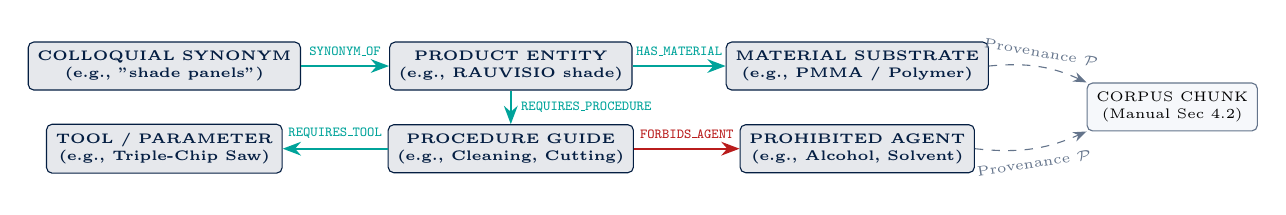
\begin{tikzpicture}[
      every node/.style={font=\tiny, align=center},
      entity/.style={rectangle, rounded corners=2pt, draw=FAUNavy, fill=FAUNavy!10, text=FAUNavy, font=\tiny\bfseries, minimum height=0.42cm, minimum width=2.1cm},
      relation/.style={->, >=Stealth, thick, color=MISTeal, font=\tiny\bfseries},
      safety/.style={->, >=Stealth, thick, color=AlertRed, font=\tiny\bfseries},
      prov/.style={dashed, ->, >=Stealth, color=NeutralMuted, font=\tiny}
    ]
      % Row 1
      \node[entity] (syn) at (0, 0) {COLLOQUIAL SYNONYM\\(e.g., "shade panels")};
      \node[entity] (prod) at (4.4, 0) {PRODUCT ENTITY\\(e.g., RAUVISIO shade)};
      \node[entity] (mat) at (8.8, 0) {MATERIAL SUBSTRATE\\(e.g., PMMA / Polymer)};
      \node[rectangle, draw=NeutralMuted, fill=NeutralLight, rounded corners=2pt, font=\tiny, align=center] (chunk) at (12.8, -0.52) {CORPUS CHUNK\\(Manual Sec 4.2)};

      % Row 2
      \node[entity] (tool) at (0, -1.05) {TOOL / PARAMETER\\(e.g., Triple-Chip Saw)};
      \node[entity] (proc) at (4.4, -1.05) {PROCEDURE GUIDE\\(e.g., Cleaning, Cutting)};
      \node[entity] (agent) at (8.8, -1.05) {PROHIBITED AGENT\\(e.g., Alcohol, Solvent)};

      % Connectors Row 1
      \draw[relation] (syn) -- node[above] {\texttt{SYNONYM\_OF}} (prod);
      \draw[relation] (prod) -- node[above] {\texttt{HAS\_MATERIAL}} (mat);

      % Connectors Row 1 -> Row 2
      \draw[relation] (prod) -- node[right] {\texttt{REQUIRES\_PROCEDURE}} (proc);

      % Connectors Row 2
      \draw[relation] (proc) -- node[above] {\texttt{REQUIRES\_TOOL}} (tool);
      \draw[safety] (proc) -- node[above] {\texttt{FORBIDS\_AGENT}} (agent);

      % Provenance arrows
      \draw[prov] (mat.east) to[bend left=15] node[above, sloped, font=\tiny] {Provenance $\mathcal{P}$} (chunk.north west);
      \draw[prov] (agent.east) to[bend right=15] node[below, sloped, font=\tiny] {Provenance $\mathcal{P}$} (chunk.south west);
    \end{tikzpicture}\par
  }
  \vspace{0.6ex}

  \begin{columns}[T]
    \begin{column}{0.49\textwidth}
      \begin{block}{Schema Entities (1,354 Nodes)}
        \centering\scriptsize
        \renewcommand{\arraystretch}{0.80}
        \setlength{\tabcolsep}{2.5pt}
        \begin{tabular}{@{}llp{4.2cm}@{}}
          \toprule
          \textbf{Entity Type} & \textbf{Count} & \textbf{Industrial REHAU Examples} \\
          \midrule
          \texttt{PRODUCT} & 428 & RAUVISIO shade, crystal, brilliant \\
          \texttt{MATERIAL} & 214 & PMMA, acrylic, PUR adhesive \\
          \texttt{PROCEDURE} & 312 & Surface cleaning, CNC sawing \\
          \texttt{PROHIBITED} & 116 & Isopropanol, solvents, abrasives \\
          \texttt{TOOL/PARAM} & 189 & Triple-chip blade, 15\,m/min feed \\
          \texttt{DEFECT/STD} & 95 & Micro-cracks, DIN EN 438 \\
          \bottomrule
        \end{tabular}
      \end{block}
    \end{column}

    \begin{column}{0.49\textwidth}
      \begin{exampleblock}{Relational Edges (1,643 Edges)}
        \centering\scriptsize
        \renewcommand{\arraystretch}{0.80}
        \setlength{\tabcolsep}{2.5pt}
        \begin{tabular}{@{}llp{4.2cm}@{}}
          \toprule
          \textbf{Relation Edge} & \textbf{Count} & \textbf{Pipeline Operational Role} \\
          \midrule
          \texttt{SYNONYM\_OF} & 582 & Maps shopfloor slang to product ID \\
          \texttt{HAS\_MATERIAL} & 341 & Links product lines to substrate \\
          \texttt{REQUIRES\_PROC} & 312 & Maps target part to authorized manual \\
          \texttt{FORBIDS\_AGENT} & 174 & High-priority safety constraint \\
          \texttt{REQUIRES\_TOOL} & 148 & Tooling specification constraint \\
          \texttt{PROVENANCE\_OF} & 86 & Exact anchor $\mathcal{P} = (\text{Doc}, \text{Sec}, \text{Page})$ \\
          \bottomrule
        \end{tabular}
      \end{exampleblock}
    \end{column}
  \end{columns}
  \note{This backup slide details the TKG schema. The ontology connects products to materials, colloquial synonyms, manufacturing procedures, and prohibited chemical agents. Most importantly, every entity and edge carries a provenance pointer directly into the corpus chunks, ensuring that knowledge graph traversal is not an abstract symbolic exercise, but directly grounds the dense cross-encoder and LLM generation in authoritative corporate documentation.}
\end{frame}

\end{document}
